\chapter{Digital Circuits}

\begin{figure}[h!]
\centering
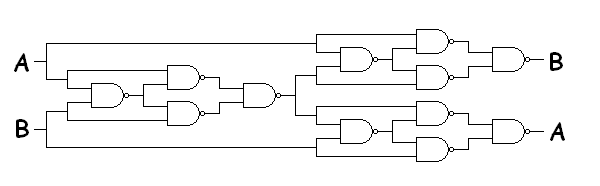
\includegraphics[width=6in]{d-ckt/d-ckt.png}
\caption{Typical digital circuit
of NAND gates.}
\label{fig-d-ckt}
\end{figure}

{\bf Digital (logic) gate:} node with
$na$ input ports and $nx$ output ports
which represents a function

\beq
f:\bool^{na}\rarrow \bool^{nx}
\;.
\label{eq-f-gate}
\eeq
{\bf Digital circuit (dcircuit)} = circuit of digital gates.


\hrule\noindent
{\bf Natural way of mapping any
dcircuit to a bnet:}
\begin{enumerate}
\item
Replace every dcircuit  gate 
described by Eq.(\ref{eq-f-gate})
with
$nx>1$ by
$nx$ gates $f_i(a^{na})$
for $i=0, 1, \ldots, nx-1$.
In other words,
replace all gates
with
multiple $nx$ output ports
by $nx$ gates with the same input ports
but a single output port.
\item
Replace
all connectors of the dcircuit
by arrows 
pointing in the direction
of the bit flow.

\item
Suppose

$a^{na}=(a_i)_{i=0, 1,\dots, na-1}$ 
where $a_i\in \bool$,

$x^{nx}=(x_i)_{i=0, 1,\dots, nx-1}$ 
where $x_i\in \bool$. 

 Replace each gate Eq.(\ref{eq-f-gate})
 by a bnet 
node with transition
prob matrix given by


\beq\color{blue}
P(x^{nx}|a^{na})=
f(a^{na})
\eeq
(By step 1, $nx=1$).

\end{enumerate}

This does not work
for digital circuits 
with feedback loops 
as occur in a flip-flop.